\documentclass[11pt]{article}

% ---------- layout & fonts ----------
\usepackage[margin=1in]{geometry}
\usepackage[T1]{fontenc}
\usepackage[utf8]{inputenc}
\usepackage{XCharter}                 % clean, readable text font
\usepackage[xcharter]{newtxmath}      % matching math font
\usepackage{microtype}
\usepackage[varqu]{zi4}               % clean monospace font (Inconsolata)
\usepackage{graphicx}
\usepackage{booktabs}
\usepackage{amsmath}
\usepackage{xcolor}
\usepackage[round]{natbib}
\usepackage[colorlinks=true, linkcolor={blue!50!black}, citecolor={blue!50!black}, urlcolor={blue!50!black}]{hyperref}
\usepackage[font=small, labelfont=bf]{caption}
\usepackage[section]{placeins}   % keeps figures/tables inside their own section

\setlength{\parindent}{0pt}
\setlength{\parskip}{0.6em}

% Boxes for the full prompt text (Appendix A)
\usepackage[most]{tcolorbox}
\newtcolorbox{promptbox}[1]{enhanced, breakable, before skip=0.8em, after skip=0.8em,
  colback=gray!4, colframe=gray!45, boxrule=0.5pt, arc=2pt,
  left=10pt, right=10pt, top=8pt, bottom=8pt,
  colbacktitle=gray!14, coltitle=black, fonttitle=\bfseries\small, title={#1},
  fontupper=\small\ttfamily\raggedright\frenchspacing, parbox=false, before upper={\setlength{\parskip}{0.7em}}}
\newcommand{\slot}[1]{\textcolor{blue!55!black}{\texttt{\{#1\}}}}

% Anything in \fillme{...} still needs input (shows up red in the PDF).

% For a double-blind submission, change \anonymousfalse to \anonymoustrue:
% this hides the author name, affiliation, and repository link.
\newif\ifanonymous
\anonymousfalse
\newcommand{\fillme}[1]{\textcolor{red}{[#1]}}

\title{\textbf{Can Small Language Models Review Research Papers?}\\[0.3em]
\large Leniency, Prompt Sensitivity, and Agreement with Human Reviewers on ICLR 2024 and 2025}
\author{\ifanonymous Anonymous Author(s)\else Pawan Chaudhary\\ \small Dakota State University\fi}
\date{October 2026}

\begin{document}
\maketitle

% =====================================================================
\begin{abstract}
\noindent
Large language models (LLMs) are starting to be used as reviewers of research papers. Before trusting one, we should know whether its verdict depends on the paper or on how the question is asked, and how it compares with a human reviewer. I tested four small open models (Qwen2.5 with 1.5, 3, and 7 billion parameters, and Phi-3.5-mini) on 400 papers submitted to ICLR, 200 from 2024 and 200 from 2025, half accepted and half rejected. Each model rated each paper's title and abstract with four prompts that ask the same question in different words. All four models give a passing score to 99--100\% of papers. When each prompt accepts its top half, 24--38\% of papers are accepted under one wording and rejected under another (random rankings would flip 88\%). The best model, Qwen2.5-7B, ranks papers with a correlation of 0.33 to the other reviewers' average on ICLR 2024, compared with 0.43 for a single human reviewer, but this falls to 0.28 against 0.52 on ICLR 2025, whose reviews and decisions were published after the models were trained; the smaller models fall close to zero. All models give higher scores to abstracts with more promotional words such as ``novel'' and ``state-of-the-art'', which human reviewers do not. A single prompt to a small LLM is therefore not a reliable paper review. All code, data, and model outputs are released.
\end{abstract}

% =====================================================================
\section{Introduction}

LLMs are now often used to judge the output of other models, and strong models agree with human judges about as often as humans agree with each other \citep{zheng2023judging}. The same idea is being applied to science. The AI Scientist \citep{lu2024aiscientist} writes complete research papers and uses an LLM reviewer to decide which ones are good, and several studies ask whether LLMs can review or give feedback on real papers \citep{liu2023reviewergpt, liang2023feedback, zhou2024reliable}. If the reviewer is unreliable, everything built on top of it is unreliable too.

There is good reason to be careful. LLM judges can be swayed by details that should not matter, such as which answer is shown first or which one is longer \citep{zheng2023judging}, and small changes to how a prompt is formatted can change an LLM's answers a lot \citep{sclar2023quantifying, mizrahi2024state}. Most work on LLM reviewers uses large commercial models and one fixed prompt. Much less is known about small open models, which are the ones students and small labs can actually run.

This paper asks three simple questions:
\begin{enumerate}
  \item If a small LLM rates the same paper using prompts that mean the same thing, does it give the same verdict?
  \item How close is its judgement to a human reviewer's?
  \item What does it reward?
\end{enumerate}

\textbf{Contributions.}
\begin{itemize}
  \item \textbf{A measurement of leniency and prompt sensitivity} for four small open models on 400 ICLR submissions: the models accept almost everything, and a large share of verdicts depend on the wording of the prompt alone (Sections~\ref{sec:leniency}--\ref{sec:stability}).
  \item \textbf{A comparison against a human ceiling}: how well one human reviewer agrees with the others, measured the same way as the models, and \textbf{a contamination check} on ICLR 2025 papers, whose reviews and decisions were released after the models were trained (Section~\ref{sec:agreement}).
  \item \textbf{Evidence about what the models reward}: their scores rise with promotional (``hype'') words, which human ratings ignore, while simple text baselines do about as well as the models at telling accepted from rejected papers (Section~\ref{sec:tracks}).
  \item \textbf{Full release} of code, prompts, model outputs, and per-score probabilities, with pinned model and data versions.
\end{itemize}

% =====================================================================
\section{Related Work}

\textbf{LLMs as judges and reviewers.}
\citet{zheng2023judging} found that GPT-4 agrees with human preferences over 80\% of the time, as often as humans agree with each other, but also that it favors answers shown first and answers that are longer. \citet{liu2023reviewergpt} tested GPT-4 on reviewing tasks such as spotting deliberately inserted errors and found it useful for some checks but unreliable as an overall judge. \citet{liang2023feedback} found that GPT-4's comments on research papers overlap with human reviewers' comments about as much as two human reviewers overlap with each other. \citet{zhou2024reliable} evaluated GPT-3.5 and GPT-4 on score prediction and review generation using ICLR reviews and concluded that the models are not yet reliable without human oversight. \citet{latona2024lottery} estimated that a noticeable share of ICLR 2024 reviews were written with AI assistance and that these reviews gave higher scores, and \citet{ye2024arewethere} showed that LLM reviewers can be manipulated by text placed in the paper. Other work builds multi-agent reviewers \citep{darcy2024marg} or simulates the whole review process with LLM agents \citep{jin2024agentreview}. The AI Scientist \citep{lu2024aiscientist} built an LLM reviewer that follows conference guidelines and reported accuracy close to human reviewers on ICLR 2022 papers. Almost all of this work uses large commercial models and a fixed prompt.

\textbf{Sensitivity to prompts.}
\citet{sclar2023quantifying} showed that formatting changes that do not alter a prompt's meaning can cause large swings in LLM accuracy, and \citet{mizrahi2024state} argue that results should be reported across many versions of a prompt, not just one. This paper applies that idea to paper reviewing, with small open models, and adds a human ceiling and a contamination check.

% =====================================================================
\section{Method}

\subsection{Papers}
ICLR publishes every submission's reviews on OpenReview. I used copies of the ICLR 2024 and ICLR 2025 data hosted on Hugging Face, pinned to fixed versions (Appendix~\ref{app:details}). A paper counts as \emph{accepted} if its decision starts with ``Accept'' and as \emph{rejected} only if its decision is exactly ``Reject''. Papers with no decision, mostly withdrawn or desk-rejected submissions (1,624 in 2024 and 2,945 in 2025), are left out. I also required at least three reviews with a numeric rating. From each year I then picked 100 accepted and 100 rejected papers at random (seed 42).

The models saw only each paper's title and abstract. For comparison I used the real decision and the reviewers' ratings, which on ICLR's scale can be 1, 3, 5, 6, 8, or 10. Accepted papers had an average rating of 6.37 (2024) and 6.58 (2025); rejected papers had 4.80 and 4.73. Each paper had about four reviews.

\subsection{Models}
I used three sizes of the Qwen2.5 family \citep{qwen2024qwen25} (1.5, 3, and 7 billion parameters) and, as a second model family, Phi-3.5-mini \citep{abdin2024phi3} (3.8 billion parameters). All are free, open, instruction-tuned models, and all were run on free Kaggle GPUs. Qwen2.5 was released in September 2024 and Phi-3.5 in August 2024, so ICLR 2024 papers, reviews, and decisions, which were public from early 2024, may be in their training data. ICLR 2025 reviews and decisions were made public from November 2024, after both models were released, so the models cannot have seen them. Some ICLR 2025 abstracts, however, were posted on arXiv before the models were trained and may have been seen.

\subsection{Prompts}
I wrote four prompts that all ask for the same thing: an overall score for the paper from 1 (reject) to 10 (accept), answered with a single number. They differ only in details that should not matter (Table~\ref{tab:prompts}; full text in Appendix~\ref{app:prompts}). A good reviewer should give the same score whichever prompt it gets.

\begin{table}[!htbp]
\centering
\begin{tabular}{ll}
\toprule
\textbf{Prompt} & \textbf{How it differs} \\
\midrule
P1 (expert) & Tells the model it is an expert reviewer; instructions come first \\
P2 (plain)  & Plain description of the task, no role \\
P3 (after)  & Instructions come \emph{after} the paper instead of before \\
P4 (terse)  & Very short, with markdown headings \\
\bottomrule
\end{tabular}
\caption{The four prompts. All ask for the same 1--10 score.}
\label{tab:prompts}
\end{table}

\subsection{Scores}
For each rating I recorded two numbers. The \emph{written score} is simply the number the model writes. It turns out to be almost always 8 or 9, which hides differences between papers. So I also used the \emph{expected score}: the model's average answer, weighted by how likely it considers each score from 1 to 10. For example, a model that is 70\% sure of 8 and 30\% sure of 7 has an expected score of 7.7. Technical details are in Appendix~\ref{app:details}.

\subsection{What I measured}
\begin{itemize}
  \item \textbf{Leniency:} the share of written scores of 6 or more. On ICLR's scale, 6 means ``marginally above the acceptance threshold''.
  \item \textbf{Consistency across prompts:} first, the \emph{mean pairwise Spearman correlation} between the rankings that two prompts produce (1 means identical rankings). Second, the \emph{verdict flip rate}: under each prompt, the top half of papers by expected score count as accepted, matching the 50/50 sample, and a paper \emph{flips} if it is accepted under one prompt and rejected under another. If the four prompts ranked papers at random, $1 - 2 \cdot 0.5^4 \approx 88\%$ of papers would flip. Third, the \emph{score shift}: how far the average score moves between the most and least generous prompt.
  \item \textbf{Agreement with humans:} the \emph{Spearman correlation} $\rho$ between a model's expected score and the average human rating (0 means no relationship), and the \emph{AUC} for telling accepted from rejected papers (0.5 is a coin flip, 1 is perfect). For the \emph{average of four}, I first average each paper's four expected scores and then compute the correlation or AUC.
  \item \textbf{Human ceiling:} the same correlation for a single human reviewer: pick one reviewer of each paper at random, correlate their rating with the average of that paper's other reviewers, and repeat 1,000 times. To compare a model on equal terms, I correlate the model's score with the same ``other reviewers'' average.
  \item \textbf{Simple baselines:} abstract length, the number of promotional words in the abstract (such as ``novel'', ``state-of-the-art'', ``significantly''; full list in Appendix~\ref{app:details}), and a word-count classifier (TF-IDF with logistic regression, cross-validated).
\end{itemize}
Ranges in brackets are 95\% bootstrap confidence intervals. Because I run many tests (4 models $\times$ 5 prompt settings $\times$ 2 measures per year), an asterisk marks results that remain significant after the Holm correction for multiple comparisons. With 200 papers per year, a single uncorrected test detects a true correlation of 0.2 81\% of the time; at the strictest Holm threshold (40 tests per year) this falls to 35\%, while a correlation of 0.3 is still detected 87\% of the time.

% =====================================================================
\section{Results}

\begin{table}[!htbp]
\centering
\small
\begin{tabular}{lccccc}
\toprule
\textbf{Model} & \textbf{Most common} & \textbf{Written} & \textbf{Prompts agree} & \textbf{Verdict flips} & \textbf{Score shift} \\
 & \textbf{written score} & \textbf{score $\ge$6} & \textbf{(mean $\rho$)} & \textbf{(random: 88\%)} & \textbf{across prompts} \\
\midrule
\multicolumn{6}{l}{\textit{ICLR 2024}} \\
Qwen2.5 1.5B & 8 (76\%) & 100\% & 0.80 & 37\% {\scriptsize[29, 44]} & 0.32 {\scriptsize[0.29, 0.35]} \\
Qwen2.5 3B & 8 (92\%) & 100\% & 0.79 & 34\% {\scriptsize[28, 42]} & 0.74 {\scriptsize[0.67, 0.81]} \\
Qwen2.5 7B & 8 (73\%) & 100\% & 0.80 & 36\% {\scriptsize[30, 44]} & 0.57 {\scriptsize[0.54, 0.61]} \\
Phi-3.5-mini & 9 (84\%) & 99\% & 0.86 & 28\% {\scriptsize[22, 35]} & 0.43 {\scriptsize[0.38, 0.50]} \\
\midrule
\multicolumn{6}{l}{\textit{ICLR 2025}} \\
Qwen2.5 1.5B & 8 (75\%) & 100\% & 0.78 & 36\% {\scriptsize[30, 43]} & 0.34 {\scriptsize[0.31, 0.37]} \\
Qwen2.5 3B & 8 (91\%) & 100\% & 0.76 & 38\% {\scriptsize[31, 46]} & 0.77 {\scriptsize[0.71, 0.84]} \\
Qwen2.5 7B & 8 (68\%) & 100\% & 0.78 & 36\% {\scriptsize[30, 44]} & 0.57 {\scriptsize[0.54, 0.60]} \\
Phi-3.5-mini & 9 (85\%) & 99\% & 0.87 & 24\% {\scriptsize[18, 32]} & 0.44 {\scriptsize[0.35, 0.53]} \\
\bottomrule
\end{tabular}

\caption{Leniency and consistency across the four prompts (200 papers per year, half truly accepted). ``Prompts agree'' is the mean Spearman correlation between the rankings of two prompts. ``Verdict flips'' is the share of papers accepted under one prompt and rejected under another when each prompt accepts its top half. ``Score shift'' is the gap between the most and least generous prompt's average expected score. Brackets: 95\% confidence intervals.}
\label{tab:stability}
\end{table}

\subsection{The models are far too generous}
\label{sec:leniency}
Every model gives a written score of 6 or more to 99--100\% of papers, although only half were accepted (Table~\ref{tab:stability}). The Qwen models write ``8'' for 68--92\% of papers, and Phi-3.5-mini writes ``9'' for 84--85\%. A reviewer that accepts everything is not really reviewing. This matches what \citet{latona2024lottery} observed in real peer review: ICLR 2024 reviews that were likely written with AI assistance gave higher scores. It also hides a second problem: if you only look at pass or fail, the models look perfectly consistent across prompts, but only because they never say no.

I can only guess at the cause. These models are trained to be helpful and agreeable, and abstracts are written to sell the paper and rarely mention its weaknesses. Both would push toward a generous score. Section~\ref{sec:tracks} gives some evidence for the second explanation.

\subsection{The verdict depends on the wording}
\label{sec:stability}
The expected score shows what the written score hides. For the Qwen models, the four prompts mostly agree on which papers are better (mean correlation 0.76--0.80), so the models are not ranking at random. But when each prompt accepts its top half, 34--38\% of papers are accepted under one wording and rejected under another, in both years. That is far below the 88\% expected from random rankings, but it means roughly one paper in three has its verdict decided by the wording of the prompt rather than its content. Phi-3.5-mini is more consistent with itself: its prompts agree more (mean correlation 0.86--0.87) and only 24--28\% of papers flip. As Section~\ref{sec:agreement} shows, it is also the model that agrees least with human reviewers, so being consistent across prompts is not the same as judging well.

Some prompt pairs disagree more than others (Appendix~\ref{app:pairwise}). For every model, the pairs that disagree most involve P3, the prompt that puts the instructions after the paper instead of before.

The prompt also moves the scores as a whole. Just by changing the wording, a Qwen model's average expected score moves by 0.32 to 0.77 points out of 10 (0.43--0.44 for Phi-3.5-mini). Since most expected scores sit in a narrow band (Figure~\ref{fig:spread}), any fixed cut-off for acceptance would depend on which prompt was used.

\begin{figure}[!htbp]
\centering
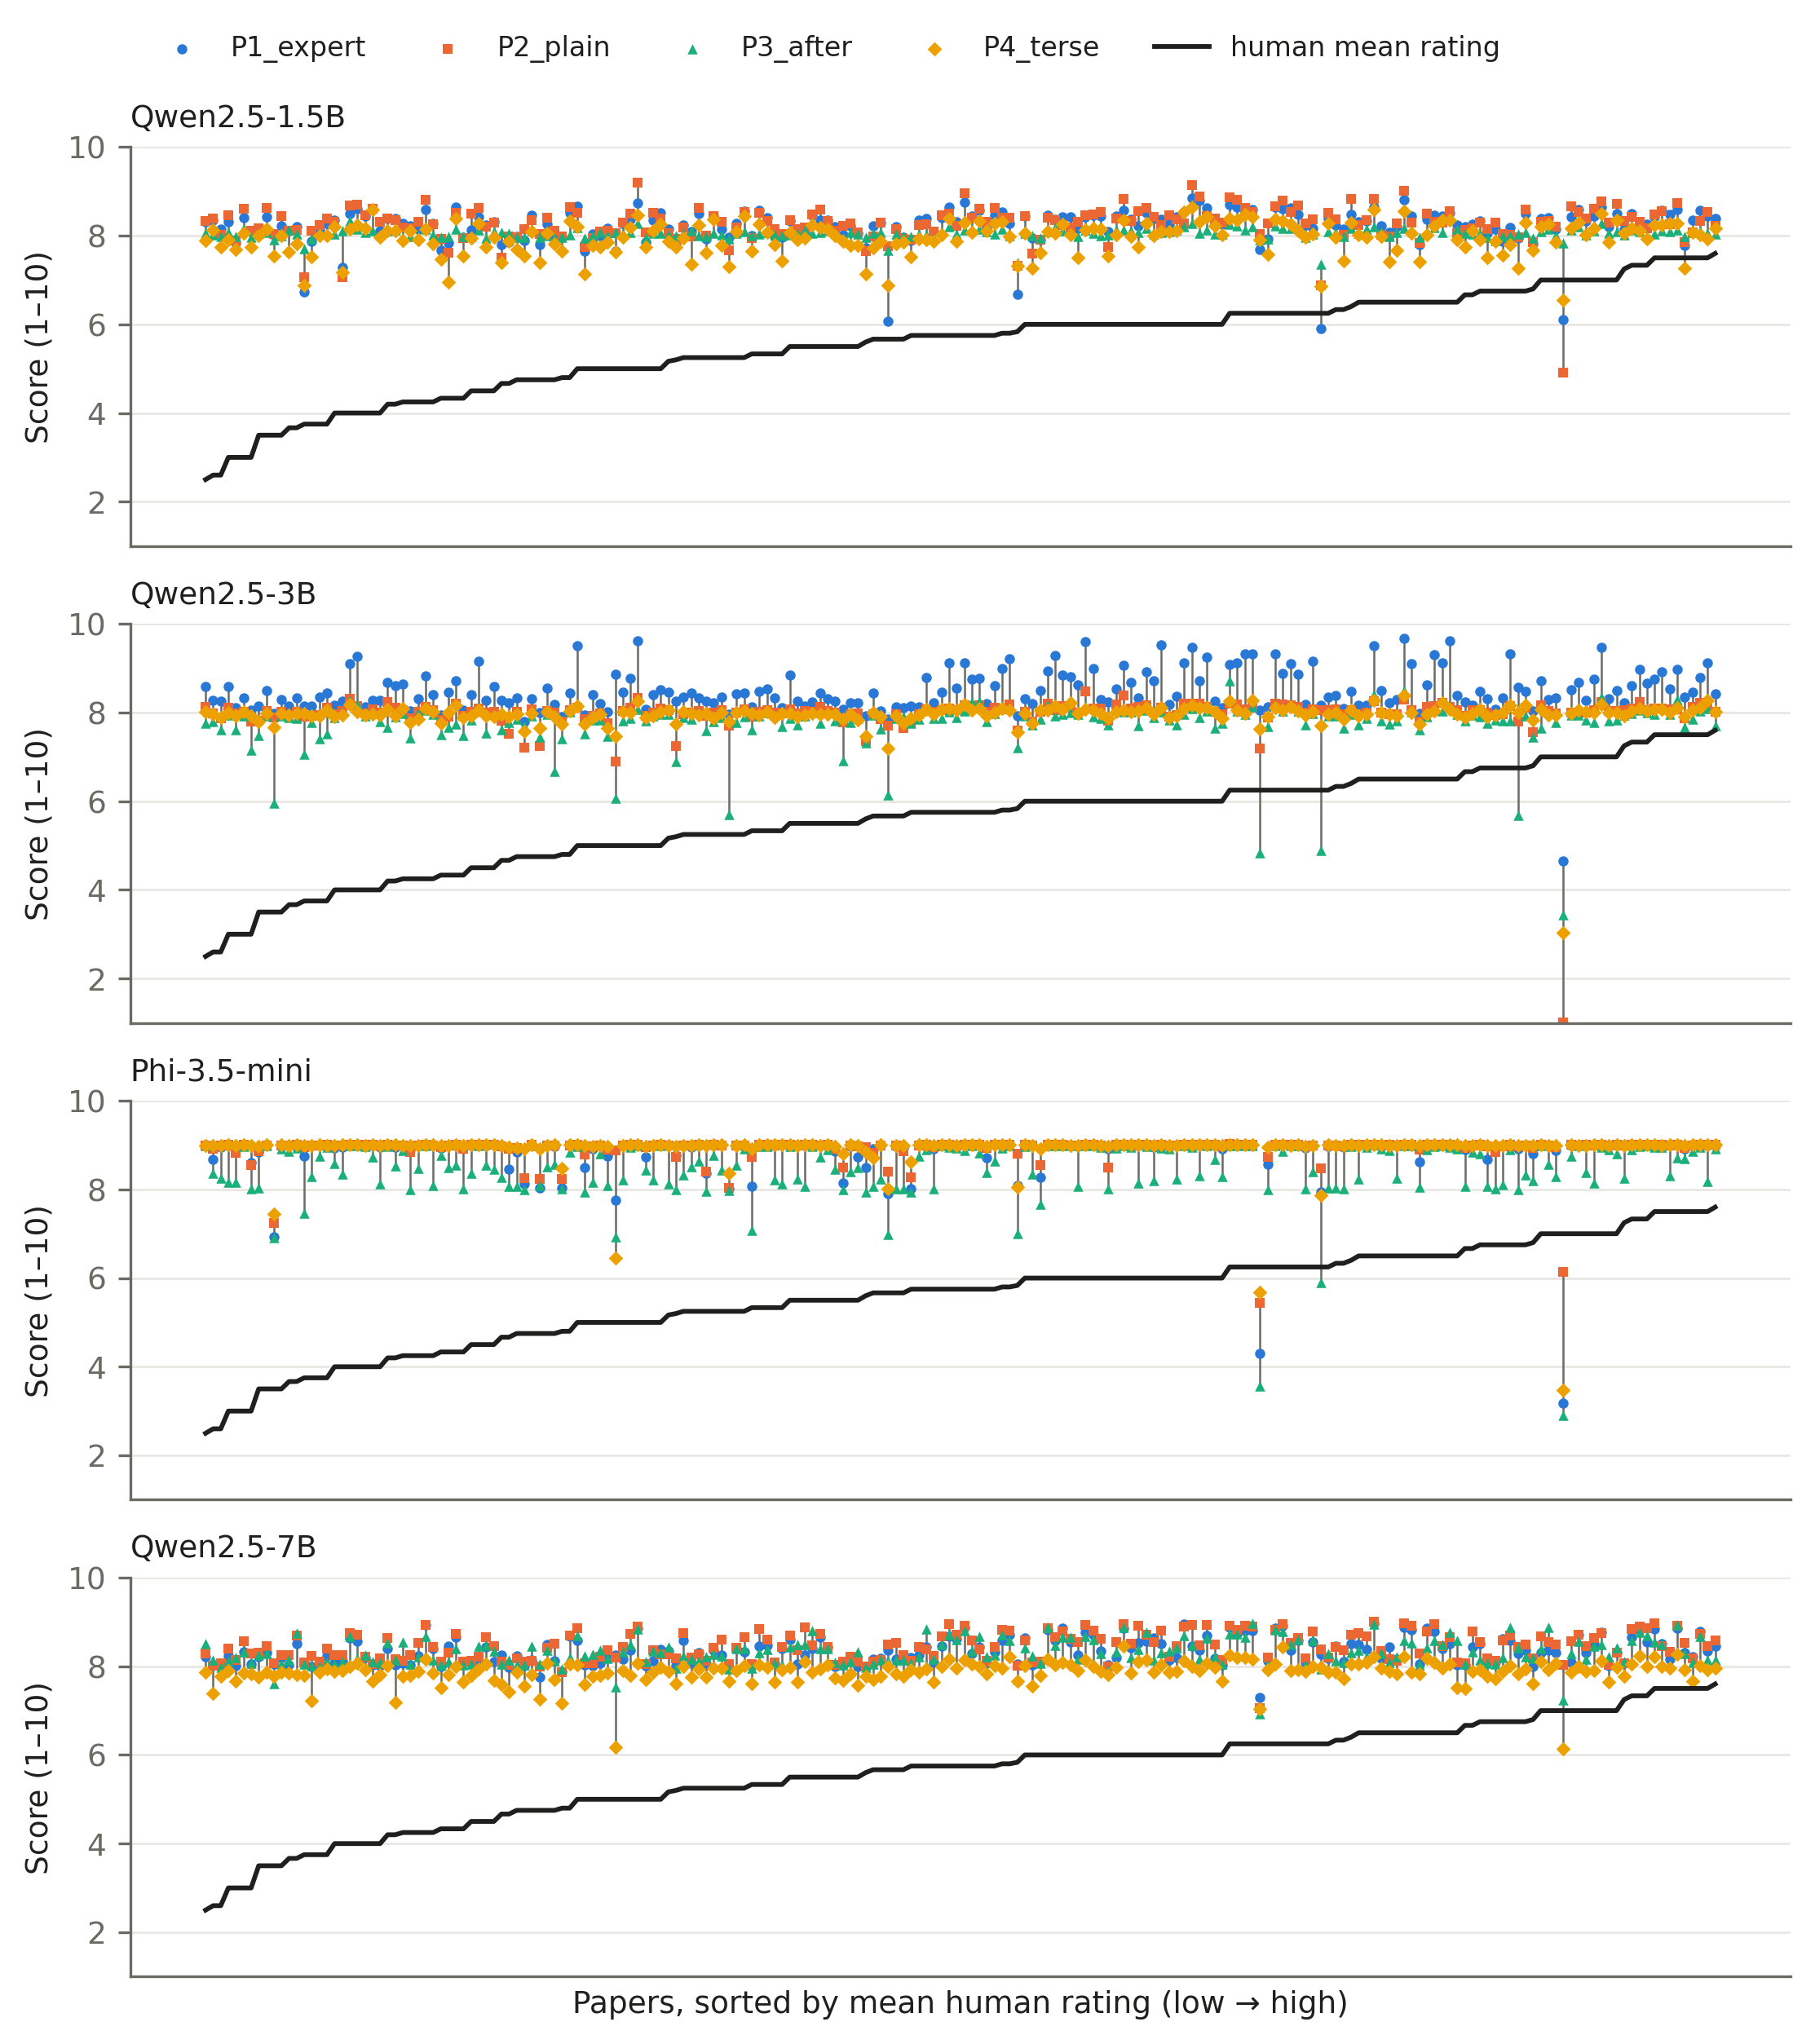
\includegraphics[width=0.95\textwidth]{figures/scores_vs_human.png}
\caption{ICLR 2024. Each column is one paper, sorted by its average human rating (black line). Colored markers are the paper's expected scores under the four prompts; the gray line spans the lowest to the highest. Model scores sit in a narrow, generous band and rise only slightly with the human rating.}
\label{fig:spread}
\end{figure}

\subsection{How close are the models to a human reviewer?}
\label{sec:agreement}

\begin{table}[!htbp]
\centering
\small
\setlength{\tabcolsep}{4pt}
\begin{tabular}{llcccc}
\toprule
 & & \multicolumn{2}{c}{\textbf{ICLR 2024}} & \multicolumn{2}{c}{\textbf{ICLR 2025}} \\
\cmidrule(lr){3-4} \cmidrule(lr){5-6}
\textbf{Model} & \textbf{Prompt} & \textbf{Correlation $\rho$} & \textbf{AUC} & \textbf{Correlation $\rho$} & \textbf{AUC} \\
\midrule
Qwen2.5 1.5B & P1 expert & 0.23 {\scriptsize[0.10, 0.35]} & 0.57 {\scriptsize[0.50, 0.66]} & 0.12 {\scriptsize[$-$0.02, 0.25]} & 0.56 {\scriptsize[0.49, 0.64]} \\
 & P2 plain & 0.14 {\scriptsize[0.00, 0.27]} & 0.55 {\scriptsize[0.47, 0.63]} & 0.09 {\scriptsize[$-$0.04, 0.23]} & 0.55 {\scriptsize[0.48, 0.64]} \\
 & P3 after & 0.20 {\scriptsize[0.05, 0.32]} & 0.57 {\scriptsize[0.49, 0.65]} & 0.05 {\scriptsize[$-$0.09, 0.17]} & 0.51 {\scriptsize[0.43, 0.59]} \\
 & P4 terse & 0.20 {\scriptsize[0.07, 0.34]} & 0.55 {\scriptsize[0.47, 0.63]} & 0.12 {\scriptsize[$-$0.01, 0.26]} & 0.57 {\scriptsize[0.50, 0.66]} \\
 & Average of four & 0.20 {\scriptsize[0.07, 0.33]} & 0.56 {\scriptsize[0.48, 0.64]} & 0.12 {\scriptsize[$-$0.01, 0.25]} & 0.56 {\scriptsize[0.48, 0.65]} \\
\midrule
Qwen2.5 3B & P1 expert & 0.27$^{*}$ {\scriptsize[0.15, 0.39]} & 0.61 {\scriptsize[0.54, 0.69]} & 0.10 {\scriptsize[$-$0.05, 0.23]} & 0.52 {\scriptsize[0.44, 0.61]} \\
 & P2 plain & 0.24$^{*}$ {\scriptsize[0.10, 0.37]} & 0.61 {\scriptsize[0.53, 0.68]} & 0.17 {\scriptsize[0.04, 0.30]} & 0.57 {\scriptsize[0.49, 0.65]} \\
 & P3 after & 0.22 {\scriptsize[0.09, 0.34]} & 0.62 {\scriptsize[0.54, 0.70]} & 0.12 {\scriptsize[$-$0.01, 0.27]} & 0.54 {\scriptsize[0.46, 0.62]} \\
 & P4 terse & 0.29$^{*}$ {\scriptsize[0.17, 0.40]} & 0.62 {\scriptsize[0.54, 0.70]} & 0.16 {\scriptsize[0.02, 0.29]} & 0.57 {\scriptsize[0.48, 0.65]} \\
 & Average of four & 0.28$^{*}$ {\scriptsize[0.14, 0.40]} & 0.62 {\scriptsize[0.55, 0.70]} & 0.13 {\scriptsize[0.00, 0.26]} & 0.55 {\scriptsize[0.47, 0.63]} \\
\midrule
Qwen2.5 7B & P1 expert & 0.35$^{*}$ {\scriptsize[0.22, 0.46]} & 0.67$^{*}$ {\scriptsize[0.59, 0.74]} & 0.25$^{*}$ {\scriptsize[0.12, 0.38]} & 0.61 {\scriptsize[0.53, 0.68]} \\
 & P2 plain & 0.32$^{*}$ {\scriptsize[0.19, 0.43]} & 0.65$^{*}$ {\scriptsize[0.57, 0.72]} & 0.30$^{*}$ {\scriptsize[0.15, 0.43]} & 0.64$^{*}$ {\scriptsize[0.57, 0.71]} \\
 & P3 after & 0.26$^{*}$ {\scriptsize[0.13, 0.39]} & 0.63 {\scriptsize[0.56, 0.70]} & 0.16 {\scriptsize[0.02, 0.30]} & 0.54 {\scriptsize[0.47, 0.63]} \\
 & P4 terse & 0.33$^{*}$ {\scriptsize[0.21, 0.45]} & 0.66$^{*}$ {\scriptsize[0.58, 0.72]} & 0.35$^{*}$ {\scriptsize[0.22, 0.47]} & 0.67$^{*}$ {\scriptsize[0.60, 0.75]} \\
 & Average of four & 0.34$^{*}$ {\scriptsize[0.22, 0.46]} & 0.67$^{*}$ {\scriptsize[0.58, 0.74]} & 0.28$^{*}$ {\scriptsize[0.15, 0.42]} & 0.62 {\scriptsize[0.54, 0.70]} \\
\midrule
Phi-3.5-mini & P1 expert & 0.22 {\scriptsize[0.09, 0.35]} & 0.59 {\scriptsize[0.51, 0.66]} & 0.12 {\scriptsize[$-$0.02, 0.25]} & 0.56 {\scriptsize[0.48, 0.64]} \\
 & P2 plain & 0.22$^{*}$ {\scriptsize[0.09, 0.33]} & 0.57 {\scriptsize[0.49, 0.65]} & 0.15 {\scriptsize[0.02, 0.28]} & 0.57 {\scriptsize[0.49, 0.65]} \\
 & P3 after & 0.14 {\scriptsize[0.01, 0.26]} & 0.57 {\scriptsize[0.49, 0.65]} & 0.00 {\scriptsize[$-$0.14, 0.12]} & 0.50 {\scriptsize[0.42, 0.57]} \\
 & P4 terse & 0.17 {\scriptsize[0.04, 0.29]} & 0.57 {\scriptsize[0.49, 0.65]} & 0.13 {\scriptsize[$-$0.02, 0.25]} & 0.57 {\scriptsize[0.49, 0.65]} \\
 & Average of four & 0.16 {\scriptsize[0.03, 0.28]} & 0.57 {\scriptsize[0.49, 0.65]} & 0.04 {\scriptsize[$-$0.10, 0.17]} & 0.52 {\scriptsize[0.45, 0.60]} \\
\midrule
Human reviewer & one vs.\ others & 0.43 {\scriptsize[0.35, 0.51]} & --- & 0.52 {\scriptsize[0.45, 0.59]} & --- \\
\bottomrule
\end{tabular}

\caption{Agreement of expected scores with human reviewers. Correlation: Spearman $\rho$ with the average human rating (0 = no relationship). AUC: accepted vs.\ rejected (0.5 = coin flip). Brackets: 95\% confidence intervals. $^{*}$: significant after Holm correction across all tests in that year. Last row: one human reviewer's rating against the average of the others.}
\label{tab:agreement}
\end{table}

\begin{table}[!htbp]
\centering
\begin{tabular}{lcc}
\toprule
\textbf{Scorer} & \textbf{ICLR 2024} & \textbf{ICLR 2025} \\
\midrule
Qwen2.5 1.5B (average of prompts) & 0.19 & 0.12 \\
Qwen2.5 3B (average of prompts) & 0.26 & 0.12 \\
Qwen2.5 7B (average of prompts) & 0.33 & 0.28 \\
Phi-3.5-mini (average of prompts) & 0.15 & 0.05 \\
\midrule
One human reviewer & 0.43 & 0.52 \\
\bottomrule
\end{tabular}

\caption{Equal-terms comparison: Spearman correlation with the average of a paper's \emph{other} reviewers, for a model (average of its four prompts) and for one randomly chosen human reviewer, averaged over random draws.}
\label{tab:ceiling}
\end{table}

On ICLR 2024 the models agree with human reviewers more than a smaller pilot study suggested (Appendix~\ref{app:history}). Agreement with the human average rises with model size, from $\rho = 0.20$ (1.5B) to $0.34$ (7B), and for Qwen2.5-3B and 7B most correlations stay significant after correcting for multiple comparisons (Table~\ref{tab:agreement}). Measured on equal terms, Qwen2.5-7B correlates 0.33 with the other reviewers' average, against 0.43 for a single human reviewer (Table~\ref{tab:ceiling}): roughly three-quarters of the way to one human reviewer. Telling accepted from rejected papers is harder: the best AUC is 0.67.

On ICLR 2025, whose reviews and decisions the models cannot have seen during training, the picture changes. Human reviewers agree with each other more (0.52), while the models agree with them less: Qwen2.5-7B falls to 0.28, and the 1.5B and 3B models fall to 0.12--0.13, with no result that survives the correction for multiple comparisons. Phi-3.5-mini agrees least with humans in both years: the average of its prompts reaches 0.16 on ICLR 2024 and 0.04 on ICLR 2025. This drop is what we would expect if part of the 2024 agreement came from the models having seen those papers or reviews during training, but it does not prove it: the confidence intervals overlap, and the two years also differ in other ways.

The prompt matters here too. On ICLR 2025, Qwen2.5-7B's correlation ranges from 0.16 (P3) to 0.35 (P4) depending only on the wording. Averaging the four prompts gives a result close to a typical prompt, not the best one. Averaging is still the safer choice: the best prompt can only be found after comparing against human ratings, and it was not the same prompt in both years.

For Phi-3.5-mini, the average is even worse than most of its single prompts (0.04 on ICLR 2025, against 0.12--0.15 for three of its four prompts). The reason is that a plain average gives more weight to prompts whose scores vary more. Phi's P3 scores are spread about twice as widely as its P2 scores (standard deviation 0.73--0.81 against 0.37), so P3, its weakest prompt, accounts for about a third of the variation in the average. Averaging the four prompts' \emph{ranks} instead of their raw scores avoids this: Phi's correlation becomes 0.20 instead of 0.16 on ICLR 2024 and 0.10 instead of 0.04 on ICLR 2025, while the Qwen models change by at most 0.02.

\begin{figure}[!htbp]
\centering
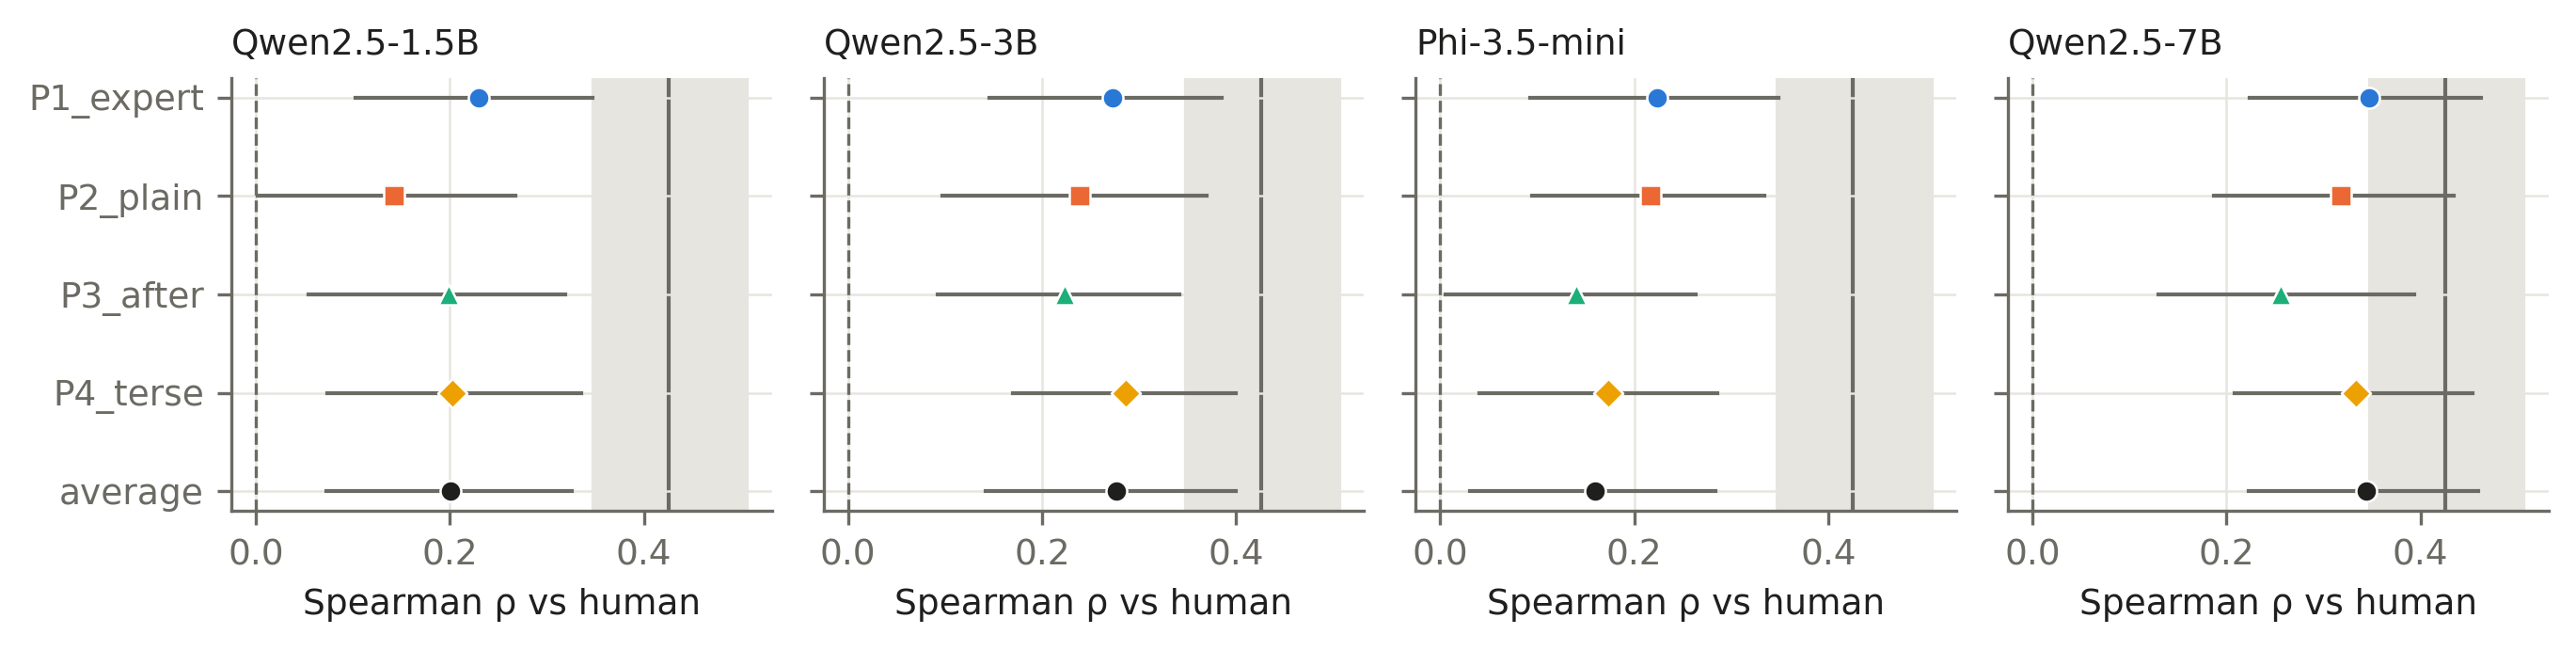
\includegraphics[width=\textwidth]{figures/agreement_vs_human.png}
\caption{ICLR 2024. Correlation between model scores and the average human rating, per prompt. Dots are estimates, lines are 95\% confidence intervals, the dashed line marks zero, and the gray band shows the range for one human reviewer against the others.}
\label{fig:agreement}
\end{figure}

\subsection{What do the models reward?}
\label{sec:tracks}

\begin{table}[!htbp]
\centering
\small
\setlength{\tabcolsep}{4pt}
\begin{tabular}{lcccccc}
\toprule
 & \multicolumn{3}{c}{\textbf{ICLR 2024}} & \multicolumn{3}{c}{\textbf{ICLR 2025}} \\
\cmidrule(lr){2-4} \cmidrule(lr){5-7}
\textbf{Correlation of \ldots\ with} & \textbf{hype rate} & \textbf{hype $|$ length} & \textbf{length} & \textbf{hype rate} & \textbf{hype $|$ length} & \textbf{length} \\
\midrule
Qwen2.5 1.5B & 0.23 & 0.31 & 0.31 & 0.24 & 0.33 & 0.24 \\
Qwen2.5 3B & 0.33 & 0.37 & 0.13 & 0.33 & 0.35 & 0.08 \\
Qwen2.5 7B & 0.24 & 0.26 & 0.13 & 0.27 & 0.31 & 0.11 \\
Phi-3.5-mini & 0.35 & 0.35 & $-$0.01 & 0.39 & 0.39 & $-$0.04 \\
\midrule
Human mean rating & 0.04 & 0.07 & 0.08 & $-$0.05 & $-$0.04 & 0.05 \\
\bottomrule
\end{tabular}

\caption{Spearman correlation of each model's score (average of the four prompts) with promotional words in the abstract, measured per 100 words (``hype rate'') and as a count with abstract length controlled for (``hype $|$ length'', a partial rank correlation), and with abstract length itself. Last row: the same correlations for the average human rating.}
\label{tab:tracks}
\end{table}

The prompts mostly agree with each other but only partly with humans, so the models must be ranking papers by something else. One clear signal is promotional language. Every model gives higher scores to abstracts that contain more words like ``novel'', ``state-of-the-art'', and ``significantly'': its score correlates 0.23 to 0.39 with the share of such words, and 0.26 to 0.39 with their count after controlling for abstract length, in both years. Human ratings are unrelated to these words (between $-0.05$ and $0.07$; Table~\ref{tab:tracks}). This is not a side effect of length: in these samples, longer abstracts do not contain more promotional words (correlation 0.05 in 2024 and 0.01 in 2025). The models are, in part, rewarding how a paper sells itself, which fits the finding of \citet{ye2024arewethere} that LLM reviewers can be steered by text written into the paper itself.

\begin{table}[!htbp]
\centering
\begin{tabular}{lcc}
\toprule
\textbf{Predictor of accept vs.\ reject} & \textbf{AUC, ICLR 2024} & \textbf{AUC, ICLR 2025} \\
\midrule
Abstract length (words) & 0.48 {\scriptsize[0.40, 0.56]} & 0.57 {\scriptsize[0.49, 0.65]} \\
Count of hype words & 0.50 {\scriptsize[0.42, 0.58]} & 0.48 {\scriptsize[0.40, 0.56]} \\
Hype words per 100 words & 0.49 {\scriptsize[0.41, 0.57]} & 0.46 {\scriptsize[0.37, 0.53]} \\
Word-count classifier (TF-IDF) & 0.54 {\scriptsize[0.50, 0.58]} & 0.63 {\scriptsize[0.59, 0.68]} \\
\midrule
Qwen2.5 1.5B (average of prompts) & 0.56 {\scriptsize[0.48, 0.64]} & 0.56 {\scriptsize[0.48, 0.65]} \\
Qwen2.5 3B (average of prompts) & 0.62 {\scriptsize[0.55, 0.70]} & 0.55 {\scriptsize[0.47, 0.63]} \\
Qwen2.5 7B (average of prompts) & 0.67 {\scriptsize[0.59, 0.74]} & 0.62 {\scriptsize[0.54, 0.70]} \\
Phi-3.5-mini (average of prompts) & 0.57 {\scriptsize[0.49, 0.65]} & 0.52 {\scriptsize[0.45, 0.60]} \\
\bottomrule
\end{tabular}

\caption{How well simple, non-LLM predictors separate accepted from rejected papers, compared with each model (AUC; 0.5 = coin flip). The word-count classifier is trained and tested with 5-fold cross-validation, repeated 10 times; brackets show the range over repeats. Other brackets: 95\% confidence intervals.}
\label{tab:baselines}
\end{table}

Simple baselines put the models' accuracy in context (Table~\ref{tab:baselines}). Abstract length and the count of promotional words are no better than a coin flip at predicting acceptance. A plain word-count classifier trained on just 160 abstracts per fold reaches an AUC of 0.54 on ICLR 2024 and 0.63 on ICLR 2025. On ICLR 2025 that is about as good as the best LLM (0.62 for the average of Qwen2.5-7B's prompts), although on ICLR 2024 the 3B and 7B models do better than the classifier. On papers whose reviews the models have not seen, much of what a small LLM reviewer gets right can also be found by counting words.

% =====================================================================
\section{Limitations}
\begin{itemize}
  \item 200 papers per year from one conference, and two model families of small size. Larger and commercial models may behave differently.
  \item The models saw only the title and abstract, not the full paper. Human reviewers read the full paper, so the comparison favors the humans.
  \item The 2024--2025 comparison is suggestive, not a controlled test of contamination: the years differ in topics, reviewers, and acceptance rates.
  \item Human ratings use a discrete scale (1, 3, 5, 6, 8, 10) while expected scores are continuous.
  \item The list of promotional words is short and hand-picked (Appendix~\ref{app:details}); a correlation with it does not show that promotional language \emph{causes} the higher scores.
  \item Several analysis choices were made after seeing earlier results; they are listed in Appendix~\ref{app:history}.
\end{itemize}

% =====================================================================
\section{Conclusion}
Small open LLMs asked to review papers accept nearly everything, change a quarter to over a third of their verdicts when the prompt is reworded, and reward promotional language that human reviewers ignore. The largest model tested reaches about three-quarters of a single human reviewer's agreement on ICLR 2024, but less on ICLR 2025, whose reviews and decisions it cannot have seen in training. Anyone using such a model as a reviewer should not rely on one prompt: test several prompts that mean the same thing, compare against human ratings on data the model has not seen, and check whether a simple baseline does just as well. Natural next steps are larger models, full papers instead of abstracts, other irrelevant changes such as section order or length, and a controlled test of whether rewriting an abstract to remove promotional words lowers the score.

\section*{Code and Data}
All code, prompts, model outputs (including the probability of every score), and analysis are available at \ifanonymous \fillme{anonymized repository link}\else \fillme{public GitHub URL, once the repository is made public}\fi.

\section*{Acknowledgments}
I used an AI assistant (Claude, by Anthropic) to help write code, run analyses, and draft and edit the text. I reviewed all of the content and take full responsibility for it.

% =====================================================================
\bibliographystyle{plainnat}
\bibliography{refs}

\clearpage
\appendix

\section{Full Prompt Text}
\label{app:prompts}
Each prompt was sent to the model as a single user message, exactly as shown below, including line breaks. The highlighted \slot{title} and \slot{abstract} are replaced with the paper's title and abstract.

\begin{promptbox}{P1 (expert) \hfill\normalfont\small Reviewer role, instructions first}
You are an expert reviewer for ICLR. Read the title and abstract below and rate the paper's overall quality on a scale from 1 (strong reject) to 10 (strong accept). Respond with a single integer only.\par
Title: \slot{title}\par
Abstract: \slot{abstract}
\end{promptbox}

\begin{promptbox}{P2 (plain) \hfill\normalfont\small Plain description, no role}
Below is a submission to the ICLR conference. As a reviewer, score it from 1 to 10, where 10 means a clear accept and 1 means a clear reject. Output just the number.\par
Title: \slot{title}\\
Abstract: \slot{abstract}
\end{promptbox}

\begin{promptbox}{P3 (after) \hfill\normalfont\small Instructions after the paper}
Title: \slot{title}\par
Abstract: \slot{abstract}\par
You are reviewing this paper for ICLR, a top machine learning conference. On a 1-10 scale (1 = strong reject, 10 = strong accept), what score would you give? Reply with one integer and nothing else.
\end{promptbox}

\begin{promptbox}{P4 (terse) \hfill\normalfont\small Short, markdown headings}
Rate this ICLR submission.\\
Scale: 1 (definitely reject) to 10 (definitely accept).\\
Format: a single integer.\par
\#\#\# Title\\
\slot{title}\par
\#\#\# Abstract\\
\slot{abstract}
\end{promptbox}

\section{Technical Details}
\label{app:details}

{\sloppy \textbf{Data versions.} \texttt{smallari/\allowbreak openreview-\allowbreak iclr2024-\allowbreak peer-\allowbreak reviews-\allowbreak RAW} at commit \texttt{259c437}, and \texttt{smallari/\allowbreak openreview-\allowbreak iclr2025-\allowbreak peer-\allowbreak reviews-\allowbreak RAW} at commit \texttt{94e63f9}. The dataset cards do not state a license; the reviews themselves are publicly posted on OpenReview. The IDs of all 400 papers are listed in the repository (\texttt{data/paper\_ids.txt}).\par}

\textbf{Models.} Qwen2.5-1.5B/3B/7B-Instruct (Hugging Face commits \texttt{989aa79}, \texttt{aa8e725}, \texttt{a09a354}) and Phi-3.5-mini-instruct (commit \texttt{2fe1924}), run in 16-bit floating point with greedy decoding and at most 8 new tokens, using PyTorch 2.11 and Transformers 5.16 on two NVIDIA T4 GPUs. Each prompt is wrapped in the model's own chat template with no system message. For Qwen, the template then inserts its default system prompt (``You are Qwen, created by Alibaba Cloud. You are a helpful assistant.''); Phi's template adds none. All runs fit within Kaggle's free weekly GPU allowance; the final run, which re-scored Phi-3.5-mini and recomputed every analysis, took 26 minutes.

\textbf{Expected score.} The expected score is
\[
  \hat{s} = \sum_{s=1}^{10} s \cdot P(s \mid \text{prompt}),
\]
using the model's probabilities for the first token of its answer, renormalized over the answers 1 to 10. Two tokenizer details matter. Both model families write numbers one digit at a time, so a first digit ``1'' could mean 1 or 10; I split it using the probability that the next token is ``0''. Phi's tokenizer also writes a space token before the digit, so for Phi the digit probabilities are read after that space token. The probability that the model's answer is a number at all is at least 98\% for every model, so the expected score reflects what the models would actually say. When a model wrote 10, its expected-score distribution put on average 77\% of its probability on 10, which supports the 1-versus-10 split.

\textbf{Promotional words.} novel, state-of-the-art, state of the art, SOTA, significantly, significant, outperform(s), superior, remarkable, unprecedented, groundbreaking, first, breakthrough, substantially, dramatically, promising, effective, efficient, robust.

\textbf{Statistics.} Correlations are Spearman rank correlations. Confidence intervals come from 1,000 bootstrap resamples of the papers. Significance uses two-sided permutation tests (2,000 permutations) with the Holm correction across all agreement tests in a year.

\section{Pairwise Flip Rates}
\label{app:pairwise}
Share of papers that flip between accept and reject for each pair of prompts, when each prompt accepts its top half (random rankings would give 50\%).

\begin{table}[!htbp]
\centering
\small
\begin{tabular}{lcccccc}
\toprule
\textbf{Model} & \textbf{P1--P2} & \textbf{P1--P3} & \textbf{P1--P4} & \textbf{P2--P3} & \textbf{P2--P4} & \textbf{P3--P4} \\
\midrule
\multicolumn{7}{l}{\textit{ICLR 2024}} \\
Qwen2.5 1.5B & 16\% & 22\% & 12\% & 27\% & 15\% & 25\% \\
Qwen2.5 3B & 17\% & 23\% & 12\% & 19\% & 18\% & 27\% \\
Qwen2.5 7B & 14\% & 21\% & 18\% & 22\% & 19\% & 23\% \\
Phi-3.5-mini & 11\% & 19\% & 10\% & 17\% & 13\% & 19\% \\
\midrule
\multicolumn{7}{l}{\textit{ICLR 2025}} \\
Qwen2.5 1.5B & 15\% & 22\% & 14\% & 25\% & 14\% & 24\% \\
Qwen2.5 3B & 15\% & 25\% & 15\% & 27\% & 15\% & 29\% \\
Qwen2.5 7B & 13\% & 24\% & 19\% & 23\% & 13\% & 26\% \\
Phi-3.5-mini & 11\% & 15\% & 10\% & 16\% & 11\% & 16\% \\
\bottomrule
\end{tabular}

\caption{Pairwise verdict flip rates. Columns name the two prompts compared.}
\label{tab:pairwise}
\end{table}

\section{Development History}
\label{app:history}
This study went through several versions, and some choices were made after seeing earlier results. For transparency:
\begin{itemize}
  \item A first pilot used 60 ICLR 2024 papers, two models, and written scores only. Because the written scores were almost all 8, I added the expected score.
  \item In the pilot, 7 of the 30 ``rejected'' papers actually had no decision (they were withdrawn or desk-rejected). The final version counts only explicit rejections.
  \item After feedback, I changed the main verdict cutoff from ICLR's real acceptance rate (31\%) to 50\% to match the balanced sample, increased the sample to 200 papers per year, and added a second model family, the ICLR 2025 contamination check, the human ceiling, and the text baselines.
  \item Qwen2.5-7B crashed twice on the same ICLR 2025 paper when prompts were scored in batches of four. Scoring one prompt at a time avoided the crash. As a result, all 7B scores for ICLR 2024 and the first 152 for ICLR 2025 were computed in batches of four, and the rest one at a time.
  \item The first full run read Phi's digit probabilities one token too early, before its space token; a sanity check (almost no probability on numbers) caught this, and Phi was re-scored with the fix. Qwen results were unaffected.
\end{itemize}

\end{document}
